\section{Introduction}

%%%%%%%%%%%%%%%%%%%%%%%%%%%%%%%%%%%%%%%%%%%%%%%%%%%%%%%%%%%%%%%%%%%%%%%%%%%

\begin{frame}
  \frametitle{Introduction To Spark}
%%TCIMACRO{To adapt the Image size}%


\includegraphics[width=\textwidth,height=7cm]{Graphics/Dist.jpg}

\end{frame}

%%%%%%%%%%%%%%%%%%%%%%%%%%%%%%%%%%%%%%%%%%%%%%%%%%%%%%%%%%%%%%%%%%%%%%%%%%%
\begin{frame}
  \frametitle{Introduction To Spark}
	\begin{itemize}[<+->]
		\item Any Big Data solution working based distributed systems.
		\item What is distributed systems in brief?
			\begin{itemize}
					\item Components interact with each other in order to achieve a common goal.
					\item Problem definition is to run a process and distribute it into Multi node.
					\item Every system has its own way to manage the cluster (distributed system). Managing the cluster including 
						\begin{itemize}
							\item How the data will be processed.
							\item How the data will be shuffling (transferring) between the nodes .
							\item Keep track of the current processing tasks.
							\item Handle the logs and long running tasks.
						\end{itemize}
			\end{itemize}
	\end{itemize}
\end{frame}

%%%%%%%%%%%%%%%%%%%%%%%%%%%%%%%%%%%%%%%%%%%%%%%%%%%%%%%%%%%%%%%%%%%%%%%%%%%

\section{What Is Apache Spark?}
\begin{frame}
  \frametitle{Introduction To Spark}
	\begin{itemize}[<+->]
		\item Apache Spark is Fast and general cluster computing engine that extends Google’s MapReduce model
		\item Write programs in terms of parallel transformations on distributed datasets.
		\item The power of supporting research in the Labs gained Spark. How? \\ \textit{Apache Spark is an open source big data processing framework built around speed, ease of use, and sophisticated analytics. It was originally developed in 2009 in UC Berkeley’s \textbf{AMPLab}, and open sourced in 2010 as an Apache project.}

	\end{itemize}%

\end{frame}

%%%%%%%%%%%%%%%%%%%%%%%%%%%%%%%%%%%%%%%%%%%%%%%%%%%%%%%%%%%%%%%%%%%%%%%%%%%%
\begin{frame}
  \frametitle{Introduction To Spark}
		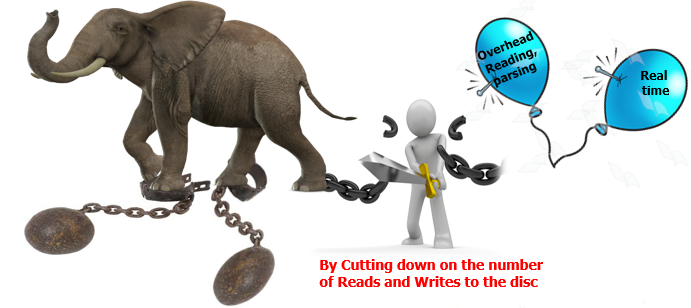
\includegraphics[width=\textwidth,height=7cm]{Graphics/Sparkvsmapreduce.png}
\end{frame}


%%%%%%%%%%%%%%%%%%%%%%%%%%%%%%%%%%%%%%%%%%%%%%%%%%%%%%%%%%%%%%%%%%%%%%%%%%%%
\begin{frame}
  \frametitle{Introduction To Spark}
	\begin{itemize}[<+->]
		\item Improves efficiency through: In-memory data sharing, General computation graphs(100x faster).
		\item Improves usability through: Rich APIs in Java, Scala, Python, Interactive shell(2-5x less code)
	\end{itemize}
\end{frame}

%%%%%%%%%%%%%%%%%%%%%%%%%%%%%%%%%%%%%%%%%%%%%%%%%%%%%%%%%%%%%%%%%%%%%%%%%%%%

\section{Example Spark vs Mapreduce on Hadoop}
\begin{frame}[fragile]
	\frametitle{Example Mapreduce on Hadoop}
%	
\includegraphics[width=3cm]{Graphics/Hadoop.PNG}

\begin{lstlisting}[style=myScalastyle, caption=Java Mapreduce Average Example]
private IntWritable one = new IntWritable(1);
private IntWritable output = new IntWritable()
proctected void map(LongWritable key,Text value, Context context) 
{String[] fields = value.split("\t");
output.set(Integer.parseInt(fields[1]));
context.write(one, output);}
IntWritable one = new IntWritable(1);
DoubleWritable average = new DoubleWritable();
protected void reduce(IntWritable key,Iterable<IntWritable> values,Context context) {
int sum = 0 ; int count = 0;
for(IntWritable value : values) {
sum += value.get(); count++;}
average.set(sum / (double) count);
context.Write(key, average);}
\end{lstlisting}

%\lstinputlisting[language=java]{"AVGExample.java"}
\end{frame}

%%%%%%%%%%%%%%%%%%%%%%%%%%%%%%%%%%%%%%%%%%%%%%%%%%%%%%%%%%%%%%%%%%%%%%%%%%%%
\begin{frame}[fragile]
	\frametitle{Example Spark on Hadoop}
	
\includegraphics[width=3cm]{Graphics/spark.jpg}
	
%	\begin{minted}{python}
	
\begin{lstlisting}[language=Python, caption=Python Spark Average Example]
	data = sc.textFile(...).split("\t")
	data.map(lambda x: (x[0], [x.[1], 1])) \
	.reduceByKey(lambda x, y: [x[0] + y[0], x[1] + y[1]]) \
	.map(lambda x: [x[0], x[1][0] / x[1][1]]) \
	.collect()	
\end{lstlisting}
%\end{minted}

\end{frame}

%%%%%%%%%%%%%%%%%%%%%%%%%%%%%%%%%%%%%%%%%%%%%%%%%%%%%%%%%%%%%%%%%%%%%%%%%%%%
\section{Downloading Spark and Getting Started.} 
\subsection{Installing Apache Spark and Scala}
\begin{frame}
	\frametitle{Installing Apache Spark and Scala}
	please refer to this article and videos below
	\begin{itemize}[<+->]
	\item \href{https://github.com/MostafaAlaa2016/Spark\_Installation}{\color{blue}Github Document}.
	\item \href{https://www.youtube.com/watch?v=WlE7RNdtfwE}{\color{blue}Youtube Video}.
	\end{itemize}
\end{frame}

